\usetikzlibrary{shapes.geometric, arrows}

\tikzstyle{block} = [rectangle, rounded corners, minimum width=3cm, minimum height=1cm, text centered, draw=black, fill=blue!30]
\tikzstyle{arrow} = [thick,->,>=stealth]

	
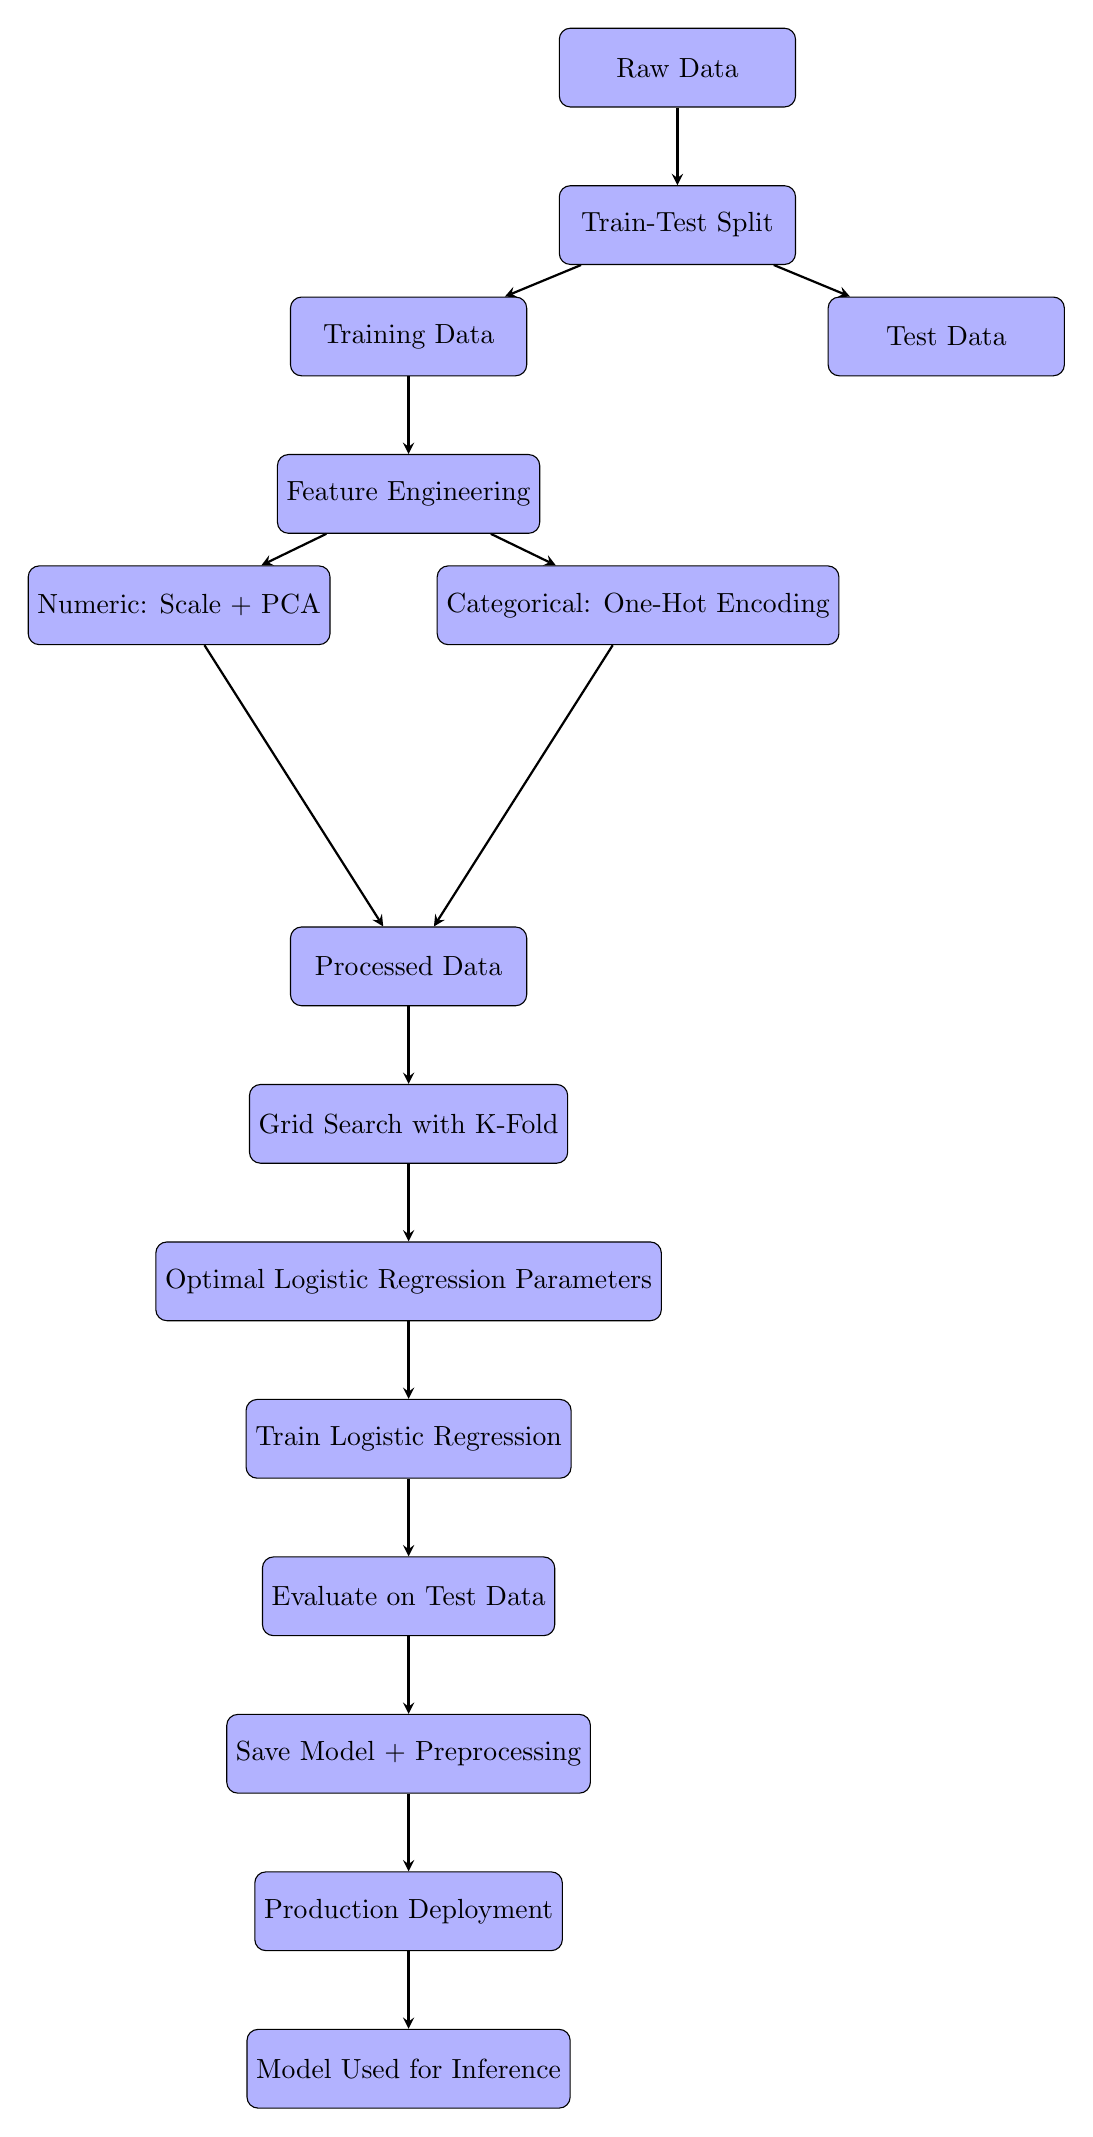
\begin{tikzpicture}[node distance=2cm]
	
	% Nodes
	\node (start) [block] {Raw Data};
	\node (split) [block, below of=start] {Train-Test Split};
	\node (train) [block, below left of=split, xshift=-2cm] {Training Data};
	\node (test) [block, below right of=split, xshift=2cm] {Test Data};
	\node (feature) [block, below of=train] {Feature Engineering};
	\node (numeric) [block, below left of=feature, xshift=-1.5cm] {Numeric: Scale + PCA};
	\node (categorical) [block, below right of=feature, xshift=1.5cm] {Categorical: One-Hot Encoding};
	\node (processed) [block, below of=feature, yshift=-4cm] {Processed Data};
	\node (gridsearch) [block, below of=processed] {Grid Search with K-Fold};
	\node (optimal) [block, below of=gridsearch] {Optimal Logistic Regression Parameters};
	\node (trainmodel) [block, below of=optimal] {Train Logistic Regression};
	\node (evaluate) [block, below of=trainmodel] {Evaluate on Test Data};
	\node (savemodel) [block, below of=evaluate] {Save Model + Preprocessing};
	\node (deploy) [block, below of=savemodel] {Production Deployment};
	\node (inference) [block, below of=deploy] {Model Used for Inference};
	
	% Arrows
	\draw [arrow] (start) -- (split);
	\draw [arrow] (split) -- (train);
	\draw [arrow] (split) -- (test);
	\draw [arrow] (train) -- (feature);
	\draw [arrow] (feature) -- (numeric);
	\draw [arrow] (feature) -- (categorical);
	\draw [arrow] (numeric) -- (processed);
	\draw [arrow] (categorical) -- (processed);
	\draw [arrow] (processed) -- (gridsearch);
	\draw [arrow] (gridsearch) -- (optimal);
	\draw [arrow] (optimal) -- (trainmodel);
	\draw [arrow] (trainmodel) -- (evaluate);
	\draw [arrow] (evaluate) -- (savemodel);
	\draw [arrow] (savemodel) -- (deploy);
	\draw [arrow] (deploy) -- (inference);
	
\end{tikzpicture}